\documentclass[10pt]{beamer}
%\documentclass[10pt, handout]{beamer}
%\setbeameroption{show notes}

%\documentclass[10pt, a4paper]{article}
%\usepackage{beamerarticle}




\mode<article>{
	
	\usepackage{hyperref}
	
}
\mode<presentation>{
	
	\usetheme{Antibes}
	\usefonttheme{professionalfonts} 
	\usefonttheme{serif} % default family is serif
	
	%\usecolortheme{spruce} %зеленая, плохой цвет в заголовках 
	%\usecolortheme{albatross} %синяя, пхоло виден черный цвет
	
}

\newcommand{\MP}[1]{\mode<presentation>{#1} }
\newcommand{\MA}[1]{\mode<article>{#1} }

\newcommand{\ABS}[1]{\left| #1 \right|}
%\newcommand{\ABS}[1]{\mid #1 \mid}

\newcommand{\HREF}[2]{{\color{blue}\underline{\href{#1}{#2}}}}

\setbeamertemplate{caption}[numbered]


%\usepackage[T2A]{fontenc}
%\usepackage[utf8]{inputenc}
%\usepackage[russian]{babel}
%\usepackage{amsmath} %математические формулы



\usepackage{ifthen}

\usepackage{tikz}
\usetikzlibrary{arrows.meta}

\usepackage{fp}
\usepackage{tikz-3dplot}
\usepackage{environ}
\usepackage{animate}




\usepackage{xcolor}
%\usepackage[left=20mm,right=20mm,top=20mm,bottom=20mm,a4paper]{geometry} %поля

\usepackage{amsmath} %математические формулы


\usepackage[e]{esvect}  %Красивая стрелочка вектора
%\let\oldvv\vv
\newcommand{\VV}[1]{\vv{#1\mathstrut}}



\usepackage{graphicx} %работа с каритнками


\usepackage{multimedia}

%Для XeLatex/+
\usepackage{polyglossia}
\setdefaultlanguage{russian}
\setotherlanguage{english}
\setkeys{russian}{babelshorthands=true}


\usepackage{fontspec}

\setmainfont{Times New Roman} [Script=Cyrillic, Mapping=tex-text,]
\setsansfont{Arial} [Script=Cyrillic, Mapping=tex-text,]
\setmonofont{Courier New} [Script=Cyrillic, Mapping=tex-text,]



\usepackage{unicode-math}
%\setmathfont{TeX Gyre Termes Math}

%\setmainfont{CMU Serif}[Script=Cyrillic, Mapping=tex-text,]
%\setsansfont{CMU Sans Serif}[Script=Cyrillic, Mapping=tex-text,]
%\setmonofont{CMU Typewriter Text}[Script=Cyrillic, Mapping=tex-text,]


%-----------------


%\usepackage{caption}
%\DeclareCaptionLabelSeparator{dot}{~---~}            %Разделитель номер рисунка
%\captionsetup[figure]{justification=centering,labelsep=dot, format=plain}                        %Подпись рис. центр
%\captionsetup[table]{justification=raggedleft,labelsep=dot, format=plain, singlelinecheck=false} %Подпись табл. слева
%\captionsetup[lstlisting]{justification=raggedleft,labelsep=dot, format=plain, singlelinecheck=false}                     %Подпись рис. центр

\usepackage{indentfirst} %отступ первой строки


\usepackage[svgnames]{xcolor}


%\usepackage{showframe}


%\usepackage{tikz}

%\usepackage[hidelinks]{hyperref}%ссылки внутри документа \ref


\setlength\abovecaptionskip{-2pt}
%\setlength\belowcaptionskip{-14pt}

\setbeamerfont{caption}{size=\scriptsize}


\def\sectionname{Раздел}
\def\subsectionname{Подраздел}


\newcommand{\TC}[3]
{
	
	
	\begin{columns}
		\begin{column}{#1\textwidth}
			#2
		\end{column}
		\begin{column}{\fpeval{1-#1}\textwidth}
			#3
		\end{column}
	\end{columns}
}

\newcommand{\TCT}[3]
{
	
	\begin{columns}[T]
		\begin{column}{#1\textwidth}
			#2
		\end{column}
		\begin{column}{\fpeval{1-#1}\textwidth}
			#3
		\end{column}
	\end{columns}
}


\newcommand{\FRAME}[2]{
	\begin{frame}
		\frametitle{#1}
		#2
	\end{frame}
}

\newcommand{\FIG}[3]
{
	\begin{figure}
		\centering
		\includegraphics[width=#3]{#1}
		\caption{#2}
	\end{figure}
}

\newcommand{\vect}[1]{\overrightarrow{#1}}


\usepackage{newfile}

\edef\LectionNumber{0}

\let\oldsection\section
\let\oldsubsection\subsection


\AtBeginDocument
{
	\newoutputstream{CONTENT}
	\openoutputfile{\LectionNumber .gvr}{CONTENT}
	
	\expandafter\addtostream{CONTENT}{\noindent\textbf{\Large\inserttitle}\unexpanded{\setcounter{SEC}{0}}\par}
}

\renewcommand{\section}[1]{
	\oldsection{#1}
	\expandafter\addtostream{CONTENT}{\noindent\hspace{2ex}\unexpanded{\hbox{\large\stepcounter{SEC}\theSEC ~ #1}}\par}
}

\renewcommand{\subsection}[1]{
	\oldsubsection{#1}
	\expandafter\addtostream{CONTENT}{\noindent\hspace{6ex}\unexpanded{\stepcounter{SUB}\theSUB ~ #1}\par}
}

%\renewcommand{\section}[1]{\MMM{#1}}

%\edef\subsection#1
{
	%\noexpand\subsection{#1}
	%
}


\author{Гаврилов Андрей Геннадьевич}
\institute{Кафедра Информационных технологий и вычислительных систем \\МГТУ~<<СТАНКИН>>}
\lecture{История компьютерной графики}{kghistory}\subtitle{Компьютерная графика}



\graphicspath{{Images/}{Images/L2/}}

\date{\today}





%\usepackage{standalone}

\setbeamersize
{
	text margin left=0.5cm,
	text margin right=0.5cm
}

\usepackage{comment}


%	\transduration{2}
%   \transfade


\renewcommand{\LectionNumber}{2}
\title{Лекция 2 \\Математические основы компьютерной графики}






\begin{document}
	 
	\makeatletter
\defbeamertemplate*{title page}{my theme}
{
	
	\hfill
	
	\begin{beamercolorbox}[wd=.9\paperwidth,center,]{title}%
		
	\end{beamercolorbox}%	
	
	\vbox to 1em {}
	
	\begin{beamercolorbox}[wd=.9\paperwidth,center,]{title}%
		\usebeamerfont{subtitle}%
		\hfill
		
		\insertsubtitle
		
		\usebeamerfont{title}%
		\inserttitle{} \\[0.5em]
		
		
		
	\end{beamercolorbox}%	
	\hfill\hfill
	
	\begin{beamercolorbox}[wd=.9\paperwidth,center,]{}%
		\usebeamerfont{author}%
		\hfill \\[0.5em]
		\insertauthor{}
		
		\vbox to 1em{}
		\usebeamerfont{institute}%
		\insertinstitute {}
		
		\vbox to 1em{}			
		{\; }\insertshortdate{}
		
	\end{beamercolorbox}%	
	\hfill\hfill
	
	\vbox to 5em{}
	
	
}
\defbeamertemplate*{footline}{my theme}{
	\leavevmode%
	\hbox{%
		\begin{beamercolorbox}[wd=.25\paperwidth,ht=2.25ex,dp=1ex,center]{author in head/foot}%
			\usebeamerfont{author in head/foot}%
			\insertauthor~~\beamer@ifempty{\insertshortinstitute}{}
		\end{beamercolorbox}%
		\begin{beamercolorbox}[wd=.65\paperwidth,ht=2.25ex,dp=1ex,center]{title in head/foot}%
			\usebeamerfont{title in head/foot}\insertshortinstitute
		\end{beamercolorbox}%
		\begin{beamercolorbox}[wd=.1\paperwidth,ht=2.25ex,dp=1ex,right]{date in head/foot}%
			\usebeamerfont{date in head/foot}\hspace*{2em}
			\insertframenumber{} / \inserttotalframenumber\hspace*{2ex}
	\end{beamercolorbox}}%
}



\makeatother






%float page top aligment
\makeatletter
\setlength{\@fptop}{0pt}
\setlength{\@fpbot}{0pt plus 1fil}
\makeatother
    
    \begin{frame}[plain]
    	
    	
    	\centering
    	Трансляция презентации (во время очных лекций).     
    		
    	
\includegraphics[width=0.5\textwidth]{qr.png} \\ ~ \\
    	
    	
    	При просмотре презентации в PDF для отображения анимаций на слайдах необходимо использовать Acrobat Reader, KDE Okular, PDF-XChange или Foxit Reader.

    \end{frame}
	
	
	\frame{\maketitle}
	
	
	
	\begin{frame}
		\tableofcontents
	\end{frame}
	
	\section{Вектор}
	\subsection{Вектора на плоскости}
	
	\frame{\sectionpage}
	
    \FRAME{Вектор}
    {
    	\TC{0.55}
    	{
    		 
			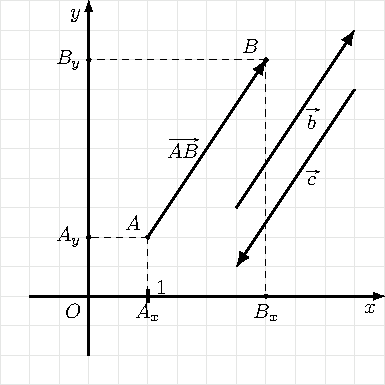
\includegraphics{vector.pdf}
    		

    	}
    	{
    		$\vv{AB}$ --- вектор.
    		
    		$ \vv{a} \equiv \vv{AB}$
    		
    		$\vv{a} = (a_x, a_y) $
    		
    		$a_x = B_x - A_x, \ a_y = B_y - A_y$
    		
	     	\hfill
	     	
	     	$\vv{a} = (2, 3)$	 \\  ~ \\
	     	
	     	$\vv{a\mathstrut} = \vv{b\mathstrut}$, \ $\vv{c\mathstrut} = -\vv{a\mathstrut}$
	     	
	     
    		
              
    		
    	}

    }
    
    
    \FRAME{Произведение вектора на скаляр}
    {
    	\TC{0.55}
    	{
    		
			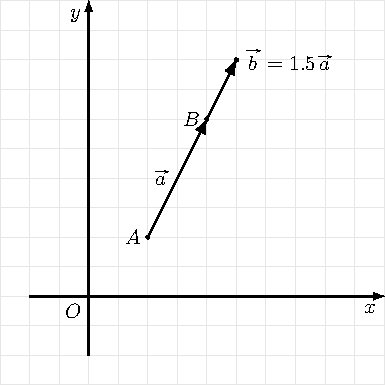
\includegraphics{normalize.pdf}
    		
    		
    	}
    	{
    		Если $\vv{b} = k\vv{a}$, 
    		
    		\hfill
    		
    		то $\vv{b}  = (ka_x, ka_y)$.
    		

    		
    		
    	}
    	
    }
    
    
    \FRAME{Произведение вектора на скаляр}
    {
    	\TC{0.55}
    	{
    		
			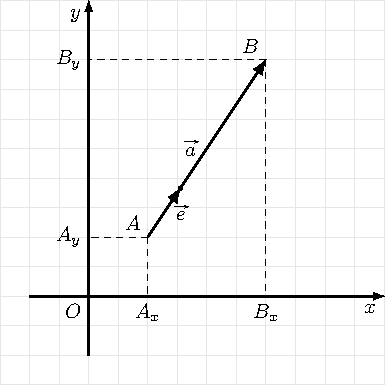
\includegraphics{veconscalar.pdf}
    		
    		
    	}
    	{
    		$d = |\vv{a}| = \sqrt{a_x^2 + a_y^2}$
    		
    		\hfill 
    		
    		Пуcть $|\vv{e}| = 1$ и $\vv{e} \uparrow \uparrow \vv{a} $.
    		
    		Тогда: \\
    		$\vv{a} = d\vv{e}$ 
    		
    		\hfill
    		
    		{\scriptsize Выделение <<векторного>> компонента (нормализация):}
    		
    		$\vv{e} = \displaystyle\frac{\vv{a}}{\sqrt{a_x^2 + a_y^2}}$
    		
    	
    	}
    	
    }
    
    
    
    
    
   \FRAME{Cумма векторов}
    {
    	\TC{0.55}
    	{
    		
    		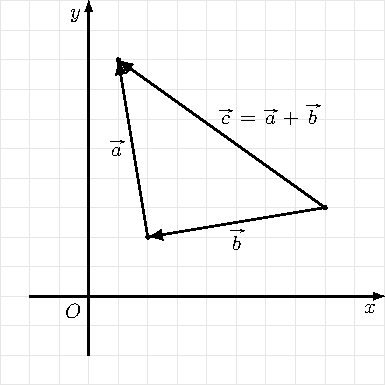
\includegraphics{vecsum.pdf}    		
    		
    	}
    	{
    		$\vv{c} = \vv{a} + \vv{b}$
    		
    		\hfill
    		
    		$c_x = a_x + b_x$\\
    		$c_y = a_y + b_y$
    		
    	}
    	
    }
    
    
    \FRAME{<<Разборка и сборка>> векторов}
    {
    	\TC{0.55}
    	{
    		
    		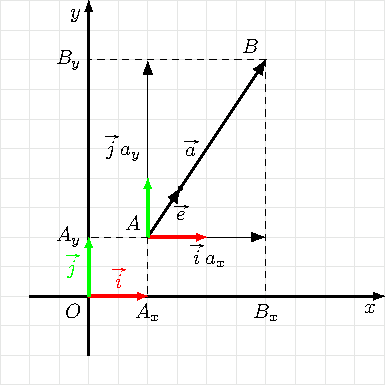
\includegraphics{veccomponents.pdf}
    		
    		
    	}
    	{
    		Орты:
    		
    		$\vv{i} = (1,0)$ и 	$\vv{j} = (0,1)$
    		
    		\hfill
    		
    		$\vv{a} = \vv{i}a_x+\vv{j}a_y$
    		
    	}
    	
    }
    
    \FRAME{Скалярное произведение векторов}
    {
    	\TC{0.55}
    	{
    		
			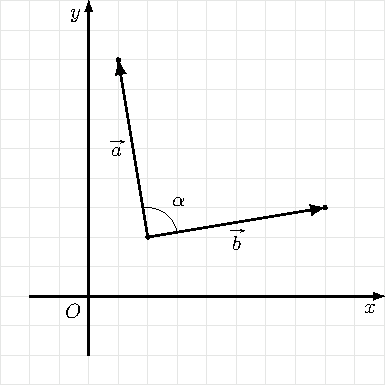
\includegraphics{scalarpr.pdf}
    		
    		
    	}
    	{
    		$\vv{a} \cdot \vv{b} = |\vect{a}||\vv{b}|\cos(\widehat{\vect{a}  \vv{b}})$ 
    		
    		\hfill
    		
    		$\vv{a} \cdot \vv{b} = a_xb_x + a_yb_y $
    		
    	}
    	
    }
	
	


\subsection{Вектора в пространстве}

\FRAME{Радиус-вектор}
{
	\TC{0.5}
	{
		
		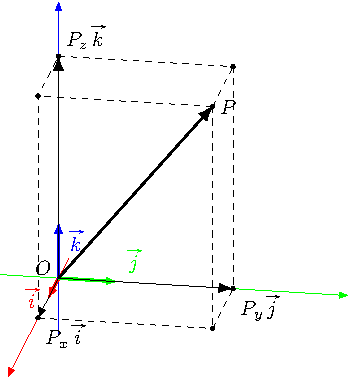
\includegraphics{pointinspace.pdf}
		
	}
	{
		$P(x,y,z) \Leftrightarrow \vv{p}=x\vv{i} + y\vv{j} + z\vv{k} $
		
		\hfill
		
		Орты:\\
		$\vv{i}=(1,0,0)$\\
		$\vv{j}=(0,1,0)$\\
		$\vv{k}=(0,0,1)$
		
		\hfill
		
		$\vv{p}$ -- радиус-вектор	
		 
		
		
	}
}

\FRAME{Векторное произведение векторов}
{
	\TC{0.55}
	{
		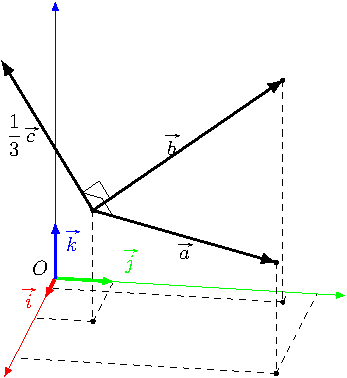
\includegraphics{vecpr.pdf}
		
		
	}
	{
		$\vv{c} = \vv{a} \times \vv{b} $
		
		$\ABS{\vv{c}} = |\vv{a}||\vv{b}|\sin( \widehat{\vv{a}\vv{b}} ) $
		
		\frame{ $ \vv{a} \times \vv{b} = - \left(\vv{b} \times \vv{a} \right) $ }
		
		\hfill	
		
		$\vv{c} = \begin{vmatrix}
			\vv{i} & \vv{j} & \vv{k} \\
			a_x & a_y & a_z          \\
			b_x & b_y & b_z          \\
		\end{vmatrix}$	
		
		
		\hfill
		
		\hfill
		
		
		$\begin{array}{rl}
			\vv{c} = & \vv{i}(a_yb_z-a_zb_y) - \\
			& - \vv{j}(a_xb_z-a_zb_x) + \\
			& + \vv{k}({a_xb_y-a_yb_x})
		\end{array}   $
	}
	
}

\MP{
	
	\FRAME{Векторное произведение в движении}
	{
		
		%\centering
		\animategraphics[autoplay,loop]{60}{Images/L2/vecpr - Copy}{0}{359} 
		
		
		
	}
}

\FRAME {Векторное произведение орт}
{
	\TC{0.4}
	{
		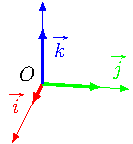
\includegraphics[page=1]{vecprort.pdf}
		
		\includegraphics[page=2]{vecprort.pdf}
	}
	{
		\begin{itemize}
			\item {Для правой системы координат: \\
			$\vv{k}=\vv{i}\times\vv{j}$ \\
			$\vv{i}=\vv{j}\times\vv{k}$ \\
			$\vv{j}=\vv{k}\times\vv{i}$}
			\item {Для левой системы координат: \\
			$\vv{k}=\vv{j}\times\vv{i}$\\
			$\vv{j}=\vv{i}\times\vv{k}$\\
			$\vv{i}=\vv{k}\times\vv{j}$\\}
		\end{itemize}
	}
}

\section {Элементы аналитической геометрии}

\frame{\sectionpage}

\subsection{Уравнение прямой}

\FRAME{Прямая}
{
	
	\TC{0.45}
	{
		
		\MP{
			
			\only<1>{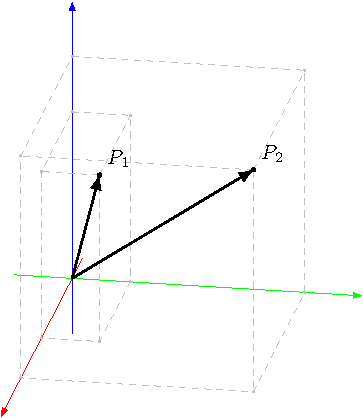
\includegraphics[page=1]{line.pdf}}
			\only<2-4>{\includegraphics[page=2]{line.pdf}}	
			\only<5>{\includegraphics[page=3]{line.pdf}}	
			\only<6->{\animategraphics[autoplay,loop]{25}{Images/L2/line_anim}{0}{282} }
		
		}
		\MA{
		
		   \only<5>{\includegraphics[page=3]{line.pdf}}
		
		}

	}
	{
		\onslide<1->{$P_1=(x_1,y_1,z_1) \Leftrightarrow \vv{p_1} $}
		\onslide<1->{$P_2=(x_2,y_2,z_2) \Leftrightarrow \vv{p_2} $\\[1em]}
		
		\onslide<2->{$\vv{p^*} = \vv{p_2} - \vv{p_1 }$}
		
		\onslide<3->{$\vv{p}(\mu) = \vv{p_1} + \mu\vv{p^* }$\\[1em]}
		
		
		\only<4-6>{$\vv{p}(0) = ?, \vv{p}(1) = ?, \vv{p}(0.5) = ?$}
		
		
		\only<7>{
				$\begin{cases}
				x-x_1 = \mu(x_2-x_1) \\ 
				y-y_1 = \mu(y_2-y_1) \\
				y-y_1 = \mu(z_2-z_1) \\
			\end{cases}
			$}

			
			
			
		{\onslide<8->{
					\begin{block}{Уравнение прямой по двум точкам}
						\small $\begin{cases}
							(x-x_1)(y_2-y_1)=(x_2-x_1)(y-y_1) \\ 
							(y-y_1)(z_2-z_1)=(y_2-y_1)(z-z_1) \\ 
							(z-z_1)(x_2-x_1)=(z_2-z_1)(x-x_1) \\ 
						\end{cases}$
				\end{block}   }   }
		
		
		
		\only<9>{\begin{block}{Параметрическая запись}
				$\vv{p} = (1 - \mu)\vv{p_1} + \mu\vv{p_2} $
			    \end{block}			} 
		
	
		
	}
}


\subsection{Плоскость}

\FRAME{Уравнение плоскости по точке и нормали}
{
	\TC{0.45}
	{
		\MP{
			\only<1>{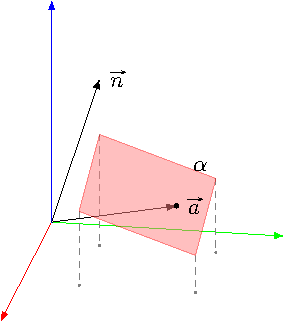
\includegraphics[page=1]{plane.pdf}}
			\only<2>{\includegraphics[page=2]{plane.pdf}}
			\only<3->{\includegraphics[page=3]{plane.pdf}}
		}
		\MA{
		
		   \includegraphics[page=3]{plane.pdf}
		
		}
	}
	{
		\onslide<1->{$ A \Leftrightarrow \vv{a}, A \in \alpha, \vv{n} \perp  \alpha$. \\[1em]}
		\onslide<2->{$ P \Leftrightarrow \vv{p}, P \in \alpha.$\\[1em]}
		\onslide<3->{$ \forall P \in \alpha:  (\vv{p}-\vv{a}) \parallel \alpha$ \uncover<4->{$\Leftrightarrow$} \\[1em]}
		\onslide<4->{ \begin{block}{Уравнение плоскости (1)}
				$\vv{n}(\vv{p}-\vv{a})=0$ 
			\end{block}}
		
		\onslide<5->{ \begin{block}{Уравнение плоскости (2)}
				$Ax+By+Cz = c$
		\end{block}
		где $P=(x,y,z), \vv{n}=(A,B,C), c=\vv{n}\vv{a}$
	    }
	}		

}

\FRAME {Уравнение плоскости по трём точкам}
{
	\TC{0.45}
	{
			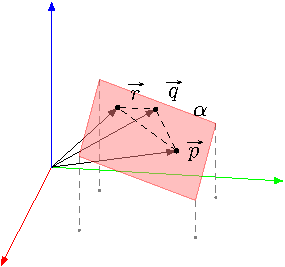
\includegraphics{plane3.pdf}
	}	
	{
		Пусть заданы три вектора $\vv{p}$, $\vv{q}$ и $\vv{r}$, не лежащие на одной прямой и определяющие плоскость $\alpha$. \\ ~ \\
		
		\pause
		
		Тогда $(\vv{p}-\vv{q})\times(\vv{p}-\vv{r}) \perp \alpha$  \\ ~ \\
		
		\pause
		
		$\forall X \in \alpha: $\\
		$\left[ (\vv{p}-\vv{q})\times(\vv{p}-\vv{r}) \right] \cdot (\vv{x} - \vv{q}) = 0 $
	}
}

\subsection{Поиск длины проекции}

\FRAME {Задача: Найти длину проекции}
{
	\TC{0.5}
	{

		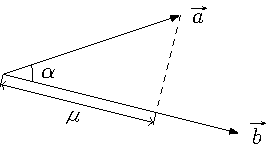
\includegraphics{projectionlength.pdf}
	}
	{
		Дано: $\vv{a}, \vv{b}$ \\
		Найти: $\mu$. \\ ~ \\
		
		\pause
		
		1. $\mu = |\vv{a}|\cos\alpha$.
		
		\pause
		
		2. $\vv{a}\cdot\vv{b} = \ABS{\vv{a}}\ABS{\vv{b}}\cos \alpha \Rightarrow $ \\
		$ \Rightarrow \cos \alpha = \displaystyle\frac{\vv{a}\cdot\vv{b}}{\ABS{\vv{a}}\ABS{\vv{b}}} $
		
		\pause
		
		3. $\displaystyle \mu=\ABS{ \vv{a} } \frac{\vv{a}\cdot\vv{b}}{\ABS{\vv{a}}\ABS{\vv{b}}} =  \vv{a} \frac{\vv{b}}{\ABS{ \vv{b} }  } $
		
			
	}
}

\subsection{Поиск расстояния до плоскости}

\FRAME {Задача: Расстояние до плоскости}
{
	\TC{0.45}
	{
		
		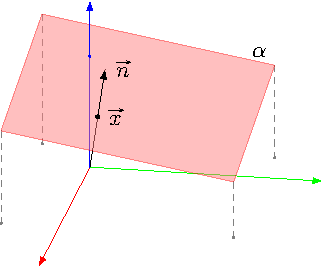
\includegraphics{plane4.pdf}
	}
	{

		Дано: Плоскость $\vv{n}\vv{x}=c$. \\
		Найти: Расстояние от т. $O$ до плоскости. \\ ~ \\
		
		\pause
		
		1. $x = \vv{p_1} + \mu\vv{p^*}$ --- прямая, проходящая через $\vv{p_1}$ в направлении $\vv{p^*}$  \\ ~ \\
		
		\pause
		
		2. $\vv{p_1} = 0, \; \vv{p^*} = \vv{n}$   \\ ~ \\
		
		\pause
		
		3. $\vv{x} = \mu\vv{n} $, \\
		 $\displaystyle\mu\vv{n}^2 = c  \Rightarrow \mu = \frac{c}{\vv{n}^2} $, \\ ~ \\
		 
		 \pause
		 
		 4. $\displaystyle\vv{x} = \frac{c}{\vv{n}^2} \vv{n} \Rightarrow $ \fbox{$\displaystyle\ABS{\vv{x}} = \frac{c}{\ABS{\vv{n}}}$}
		 
		
	}
}

\subsection{Повороты}

\FRAME{Направляющие косинусы}
{
	\TC{0.4}{
		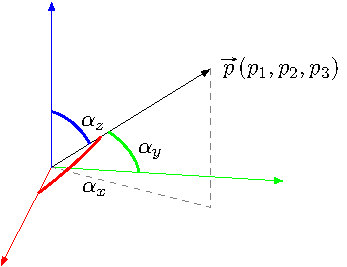
\includegraphics{cos.pdf}
	}{
		Пусть $\vv{p} = (p_1, p_2, p_3)$ и $\widehat{(\vv{p}, OX)} = \alpha_x$, $\widehat{(\vv{p}, OY)} = \alpha_y$, $\widehat{(\vv{p}, OZ)} = \alpha_z$. \\ ~ \\
		
		\begin{block}{Направляющие косинусы}
					$ \displaystyle \cos \alpha_x= \frac{p_1}{\ABS{\vv{p}}}, \; \cos \alpha_y= \frac{p_2}{\ABS{\vv{p}}}, \;  \cos \alpha_z= \frac{p_3}{\ABS{\vv{p}}} $
		\end{block}
		
		$\cos^2 \alpha_x + \cos^2 \alpha_y + \cos^2 \alpha_z =1$ \\ ~ \\
		
		$\cos \alpha_x : \cos \alpha_y : \cos \alpha_z = p_1 : p_2 : p_3$ \\ ~ \\
		
		Если $\ABS{\vv{p}} = 1$, то $\cos \alpha_x = p_1$, $\cos \alpha_y = p_2$, $\cos \alpha_z = p_3$.
	}
}

\subsection{Принадлежность точки треугольнику}

\FRAME {Задача: Находится ли точка внутри треугольника?}
{
	\TC{0.35}
	{
		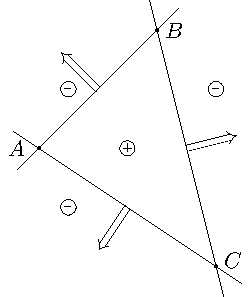
\includegraphics{triangle.pdf} \\ ~ \\
	}
	{
		Метод 1 \\ ~ \\
		
		$f(x,y)=Lx+My+N$ --- прямая, $\vv{n}=(L,M) \perp f$. \\ ~ \\
		
		\pause
		
		Решение: Проверка знака функций прямых $f(x,y)$ для всех сторон треугольника и его вершин.
	}
}

\FRAME {Задача: Находится ли точка внутри треугольника?}
{
	\TC{0.55}
	{
		\only<1>{ \includegraphics[page=2]{triangle2.pdf} }
		\only<2>{ 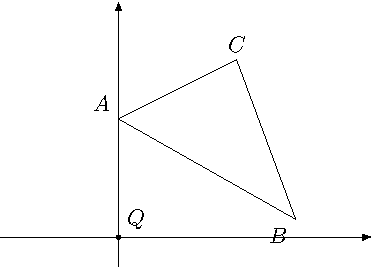
\includegraphics[page=1]{triangle2.pdf} }
		\only<3>{ \includegraphics[page=4]{triangle2.pdf} }
		\only<4>{ \includegraphics[page=3]{triangle2.pdf} }
	}
	{
		Метод 2 \\ ~ \\
		
		1. Преобразуем треугольник так, чтобы $Q$ совпадала с началом координат, а одна из его вершин лежала на оси $OY$. 	\\ ~ \\	
		
		\pause
		
		
		2. Если координаты $x$ других вершин одного знака, то  $Q$ лежит вне треугольника, в противном случае  --- внутри. 	

	}
}

\FRAME {Задача: Находится ли точка внутри треугольника?}
{
	\TC{0.45}
	{
		\includegraphics[page=5]{triangle2.pdf} 

	}
	{
		Метод 3 \\ ~ \\
		
		1. Найти преобразование $q: \triangle ABC \xrightarrow{q} \triangle A'B'C'$ и $A'=(0,0), B'=(1,0), C'=(0,1) $. 	\\ ~ \\
		
		\pause
		2. Применить это преобразование к $Q$: $Q \xrightarrow{q} Q'$. \\ ~ \\
		
		\pause
		
		3. Если $Q '_x+Q '_y < 1$, точка лежит внутри треугольника.
		
	}
	
	
}

	
\end{document}